\documentclass[11pt,compress,t,notes=noshow]{beamer}
\usepackage[]{graphicx}\usepackage[]{color}
% maxwidth is the original width if it is less than linewidth
% otherwise use linewidth (to make sure the graphics do not exceed the margin)
\makeatletter
\def\maxwidth{ %
  \ifdim\Gin@nat@width>\linewidth
    \linewidth
  \else
    \Gin@nat@width
  \fi
}
\makeatother

\definecolor{fgcolor}{rgb}{0.345, 0.345, 0.345}
\newcommand{\hlnum}[1]{\textcolor[rgb]{0.686,0.059,0.569}{#1}}%
\newcommand{\hlstr}[1]{\textcolor[rgb]{0.192,0.494,0.8}{#1}}%
\newcommand{\hlcom}[1]{\textcolor[rgb]{0.678,0.584,0.686}{\textit{#1}}}%
\newcommand{\hlopt}[1]{\textcolor[rgb]{0,0,0}{#1}}%
\newcommand{\hlstd}[1]{\textcolor[rgb]{0.345,0.345,0.345}{#1}}%
\newcommand{\hlkwa}[1]{\textcolor[rgb]{0.161,0.373,0.58}{\textbf{#1}}}%
\newcommand{\hlkwb}[1]{\textcolor[rgb]{0.69,0.353,0.396}{#1}}%
\newcommand{\hlkwc}[1]{\textcolor[rgb]{0.333,0.667,0.333}{#1}}%
\newcommand{\hlkwd}[1]{\textcolor[rgb]{0.737,0.353,0.396}{\textbf{#1}}}%
\let\hlipl\hlkwb

\usepackage{framed}
\makeatletter
\newenvironment{kframe}{%
 \def\at@end@of@kframe{}%
 \ifinner\ifhmode%
  \def\at@end@of@kframe{\end{minipage}}%
  \begin{minipage}{\columnwidth}%
 \fi\fi%
 \def\FrameCommand##1{\hskip\@totalleftmargin \hskip-\fboxsep
 \colorbox{shadecolor}{##1}\hskip-\fboxsep
     % There is no \\@totalrightmargin, so:
     \hskip-\linewidth \hskip-\@totalleftmargin \hskip\columnwidth}%
 \MakeFramed {\advance\hsize-\width
   \@totalleftmargin\z@ \linewidth\hsize
   \@setminipage}}%
 {\par\unskip\endMakeFramed%
 \at@end@of@kframe}
\makeatother

\definecolor{shadecolor}{rgb}{.97, .97, .97}
\definecolor{messagecolor}{rgb}{0, 0, 0}
\definecolor{warningcolor}{rgb}{1, 0, 1}
\definecolor{errorcolor}{rgb}{1, 0, 0}
\newenvironment{knitrout}{}{} % an empty environment to be redefined in TeX

\usepackage{alltt}
\newcommand{\SweaveOpts}[1]{}  % do not interfere with LaTeX
\newcommand{\SweaveInput}[1]{} % because they are not real TeX commands
\newcommand{\Sexpr}[1]{}       % will only be parsed by R



\usepackage[english]{babel}
\usepackage{dsfont}
\newcommand\bmmax{2}
\usepackage{bm}
\usepackage{bbm}
\usepackage{verbatim}
\usepackage{amsmath}
\usepackage{amsfonts}
\usepackage{csquotes}
\usepackage{multirow}
\usepackage{longtable}
\usepackage{enumerate}
\usepackage[absolute,overlay]{textpos}
\usepackage{psfrag}
\usepackage{algorithm}
\usepackage{algorithmicx}
\usepackage{algpseudocode}
\usepackage{eqnarray}
\usepackage{multimedia}
\usepackage{media9}
\usepackage{arydshln}
\usepackage{tabularx}
\usepackage{placeins}
\usepackage{tikz}
\usepackage{setspace}
\usepackage{wrapfig}
\usepackage{tcolorbox}
\usepackage[export]{adjustbox}
\usepackage{siunitx}
\usetikzlibrary{shapes,arrows,automata,positioning,calc}
\tikzset{
  %Define standard arrow tip
  >=stealth',
  %Define style for boxes
  punkt/.style={
    rectangle,
    rounded corners,
    draw=black, very thick,
    text width=6.5em,
    minimum height=2em,
    text centered},
  % Define arrow style
  pil/.style={
    ->,
    thick,
    shorten <=2pt,
    shorten >=2pt,}
}
\usepackage{subfig}

%new environments

\newenvironment{vbframe}  %frame with breaks and verbatim
{
 \begin{frame}[containsverbatim,allowframebreaks]
}
{
\end{frame}
}

\newenvironment{vframe}  %frame with verbatim without breaks (to avoid numbering one slided frames)
{
 \begin{frame}[containsverbatim]
}
{
\end{frame}
}

\newenvironment{blocki}[1]   % itemize block
{
 \begin{block}{#1}\begin{itemize}
}
{
\end{itemize}\end{block}
}

\newenvironment{fragileframe}[2]{  %fragile frame with framebreaks
\begin{frame}[allowframebreaks, fragile, environment = fragileframe]
\frametitle{#1}
#2}
{\end{frame}}


\newcommand{\myframe}[2]{  %short for frame with framebreaks
\begin{frame}[allowframebreaks]
\frametitle{#1}
#2
\end{frame}}

\newcommand{\remark}[1]{
  \textbf{Remark:} #1
}

%%%%%%%%%%%%%%%%%%%%%%%%%%%%%%%%%%%%%%%%%%%%%%%%%%%%%%%%%%%%%%%%%%%%%%%%%%%%%%%

% basic latex stuff
\newcommand{\pkg}[1]{{\fontseries{b}\selectfont #1}} %fontstyle for R packages
\newcommand{\lz}{\vspace{0.5cm}} %vertical space
\newcommand{\dlz}{\vspace{1cm}} %double vertical space
\newcommand{\oneliner}[1] % Oneliner for important statements
{\begin{block}{}\begin{center}\begin{Large}#1\end{Large}\end{center}\end{block}}


%\usetheme{lmu-lecture}
\usepackage{../style/lmu-lecture}

\let\code=\texttt
\let\proglang=\textsf

\setkeys{Gin}{width=0.9\textwidth}



\title{Deep Learning}
\author{Mina Rezaei}
\institute{Department of Statistics -- LMU Munich}
\date{Winter Semester 2020}

\setbeamertemplate{frametitle}{\expandafter\uppercase\expandafter\insertframetitle}



\begin{document}


\input{../../latex-math/basic-math}

\lecturechapter{10}{RNNs Applications}
\lecture{Deeplearning}

\begin{frame}
\frametitle{Lecture outline}
\tableofcontents
\end{frame}

\section{Application: Language modelling}

%\begin{frame} {RNNs - Use Case specific architectures}
%
%  \small{RNNs are very versatile. They can be applied to a wide range of tasks.
%  
%  \begin{figure}
%      \centering
%      \scalebox{0.9}{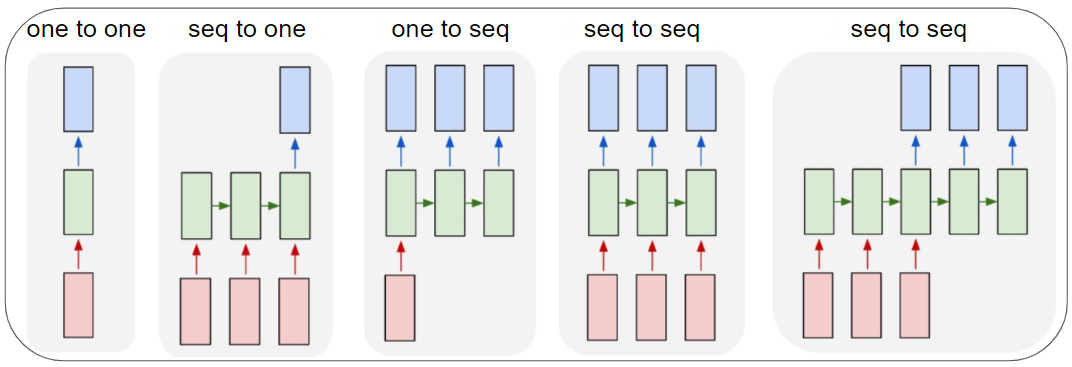
\includegraphics{plots/usecase_1.png}}
%      \tiny{\\credit: Andrej Karpathy}
%      \caption{\footnotesize {RNNs can be used in tasks that involve multiple inputs and/or multiple outputs. }}
%  \end{figure}
%  Examples:}
%  \begin{itemize}
%    \item \small{Many-to-One : Sentiment analysis, document classification.
%    \item One-to-Many : Image captioning.
%    \item Many-to-Many : Language modelling, machine translation, time-series prediction.}
%  \end{itemize}
%\end{frame}


\begin{frame}

\vspace{15mm}
\hspace{25mm} \textbf{\LARGE{Seq-to-Seq (Type I)}}
\begin{figure}
      \centering
      \scalebox{0.9}{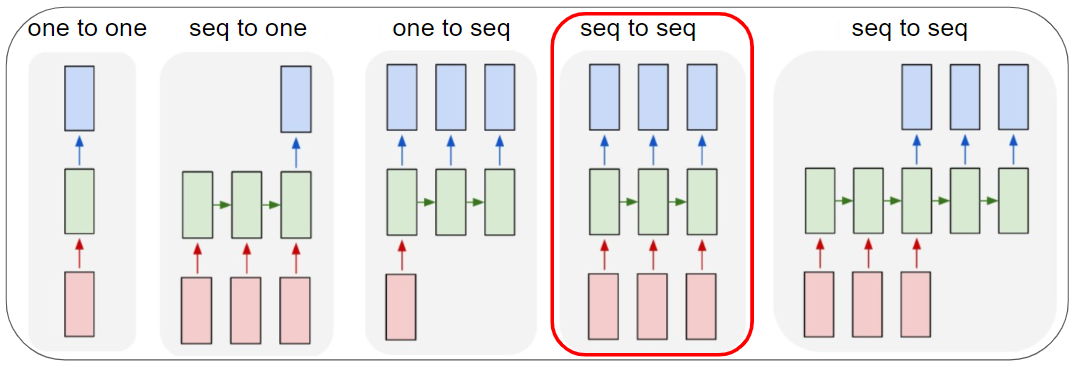
\includegraphics{plots/usecase_2.png}}
      \tiny{\\Credit: Andrej Karpathy}
  \end{figure}
  
\end{frame}

%%%%%%%%%%%%%%%%%%%%%%%%%%%%%%%%%%%%%%%%%%%%%%%%%%%%%%%%%%%%%%%%%%
% \begin{vbframe}{RNNs - Sentiment Analysis}
%   \begin{itemize}
%     \item Suppose we would like to train a model to read a sentence and extract the year the narrator went to munich:
%     \begin{itemize}
%       %\item \enquote{$\underbrace{\text{I went to Munich in 2009}}_{\text{24 characters}}$}
%       %\item[]
%       %\item \enquote{$\underbrace{\text{In 2009, I went to Munich}}_{\text{25 characters}}$}
%       \item \enquote{I went to Munich in 2009}
%       \item \enquote{In 2009, I went to Munich}
%     \end{itemize}
%     \item A standard dense network would have separate parameters for each input feature. Thus it would need to learn all of the rules of the language separately at each position in the sentence!
%       \item To overcome this issue, we introduce \textbf{recurrent neural networks}!
%       \item In order to go from a standard dense to such a recurrent net, we need to take advantage of an idea we have already learned in the CNN chapter: \textbf{parameter sharing}.
%   \end{itemize}
% \framebreak
%   \begin{itemize}
%     \item Parameter sharing enables us to apply the model to examples of different forms (here: different lengths)!
%     \item If we had separate parameters for each value of the input data, we could not generalize to sequence lengths not seen during training.
%     \item Parameter sharing is specifically important, when a particular piece of information might occur at multiple positions within the input sequence.
%     % \item Recurrent networks share parameters in a different way than CNNs: 
%     % \begin{itemize}
%     %   \item[] each member of the output is a function of the previous members of the output.
%     %   \item[] each member of the output is produced using the same update rule applied to the previous outputs
%     % \end{itemize}
%   \end{itemize}
% \end{vbframe}
%%%%%%%%%%%%%%%%%%%%%%%%%%%%%%%%%%%%%%%%%%%%%%%%%%%%%%%%%%%%%%%%%%
%%%%%%%%%%%%%%%%%%%%%%%%%%%%%%%%%%%%%%%%%%%%%%%%%%%%%%%%%%%%%%%%%%
\begin{vbframe}{RNNS - Language Modelling}
  \begin{itemize}
    \item In an earlier example, we built a 'sequence-to-one' RNN model to perform 'sentiment analysis'.
    \item Another common task in Natural Language Processing (NLP) is \textbf{'language modelling'}.
    \item Input: word/character, encoded as a one-hot vector.
    \item Output: probability distribution over words/characters given previous words $$\P(y^{[1]}, \dots, y^{[\tau]}) = \displaystyle \prod_{i=1}^{\tau} \P(y^{[i]}|y^{[1]}, \dots, y^{[i-1]})$$
    \item[] $\to$ given a sequence of previous characters, ask the RNN to model the probability distribution of the next character in the sequence!
    % \item[]
    % \item[]
    % \item[]
    % \item Time to formalize RNNs...
   \end{itemize}
\end{vbframe}



%%%%%%%%%%%%%%%%%%%%%%%%%%%%%%%%%%%%%%%%%%%%%%%%%%%%%%%%%%%%%%%%%%
%%%%%%%%%%%%%%%%%%%%%%%%%%%%%%%%%%%%%%%%%%%%%%%%%%%%%%%%%%%%%%%%%%
\begin{vbframe}{RNNS - Language Modelling}
  \begin{itemize}
  \item In this example, we will feed the characters in the word "hello" one at a time to a 'seq-to-seq' RNN.
  \item For the sake of the visualization, the characters "h", "e", "l" and "o" are one-hot coded as a vectors of length 4 and the output layer only has 4 neurons, one for each character (we ignore the <eos> token).
  \item At each time step, the RNN has to output a probability distribution (softmax) over the 4 possible characters that might follow the current input.
  \item Naturally, if the RNN has been trained on words in the English language: 
    \begin{itemize}
      \item The probability of \enquote{e} should be likely, given the context of \enquote{h}.
      \item \enquote{l} should be likely in the context of \enquote{he}.
      \item \enquote{l} should \textbf{also} be likely, given the context of \enquote{hel}.
      \item and, finally, \enquote{o} should be likely, given the context of \enquote{hell}.
    \end{itemize}
  \end{itemize}
\end{vbframe}
%%%%%%%%%%%%%%%%%%%%%%%%%%%%%%%%%%%%%%%%%%%%%%%%%%%%%%%%%%%%%%%%%%
%%%%%%%%%%%%%%%%%%%%%%%%%%%%%%%%%%%%%%%%%%%%%%%%%%%%%%%%%%%%%%%%%%
\frame{
\frametitle{RNNS - Language Modelling}
  \begin{figure}
      \only<1>{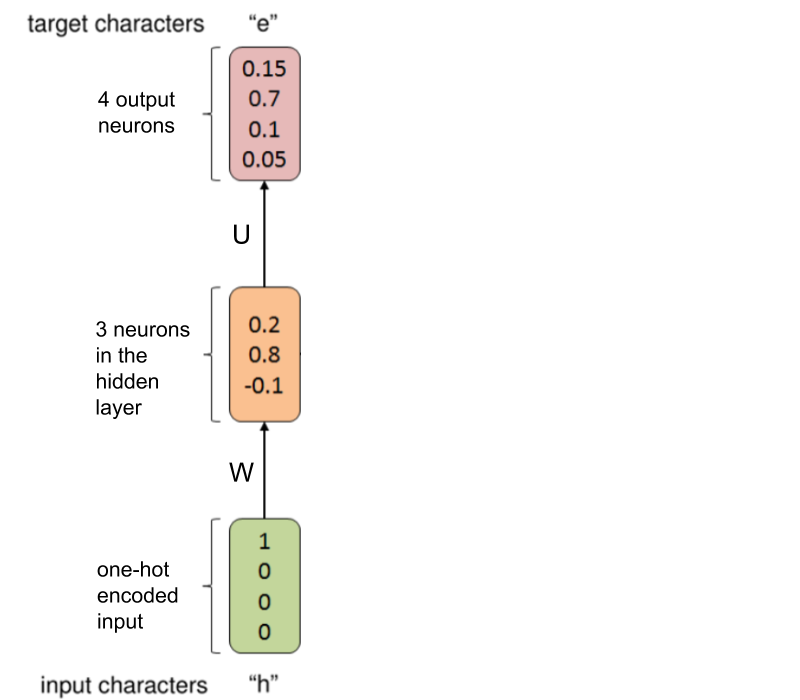
\includegraphics[width=6.5cm]{plots/m2many1.png}}%
      \only<2>{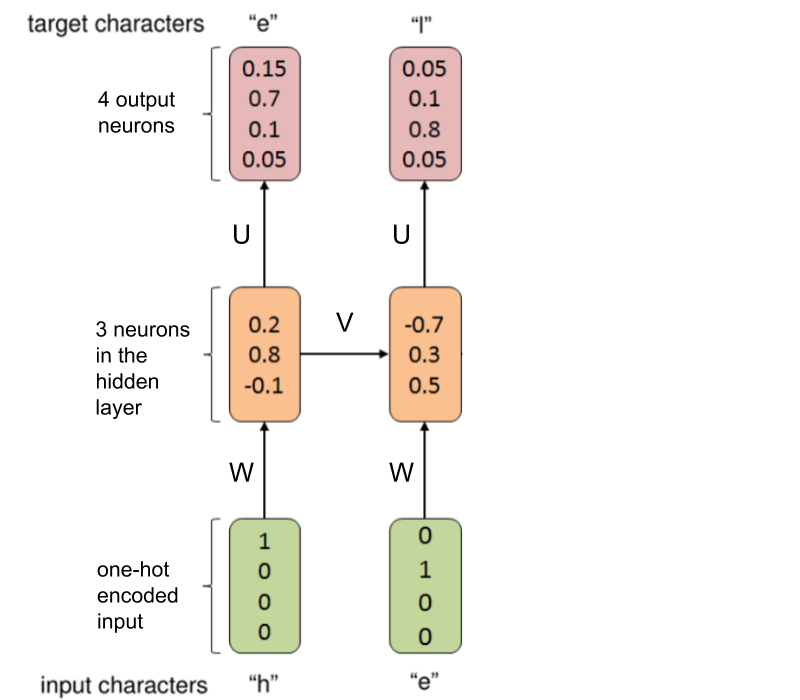
\includegraphics[width=6.5cm]{plots/m2many2.png}}%
      \only<3>{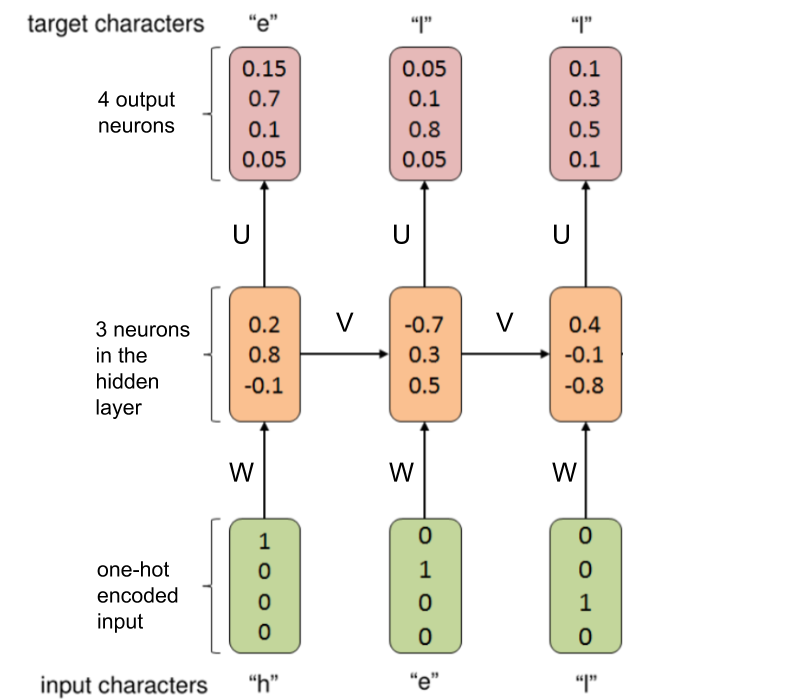
\includegraphics[width=6.5cm]{plots/m2many3.png}}%
      \only<4>{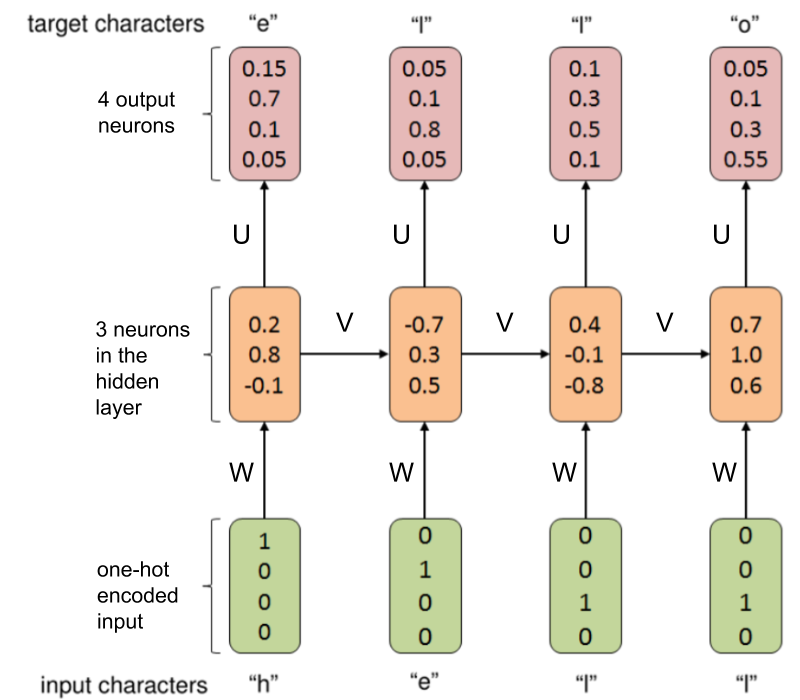
\includegraphics[width=6.5cm]{plots/m2many4.png}}%
      \only<5>{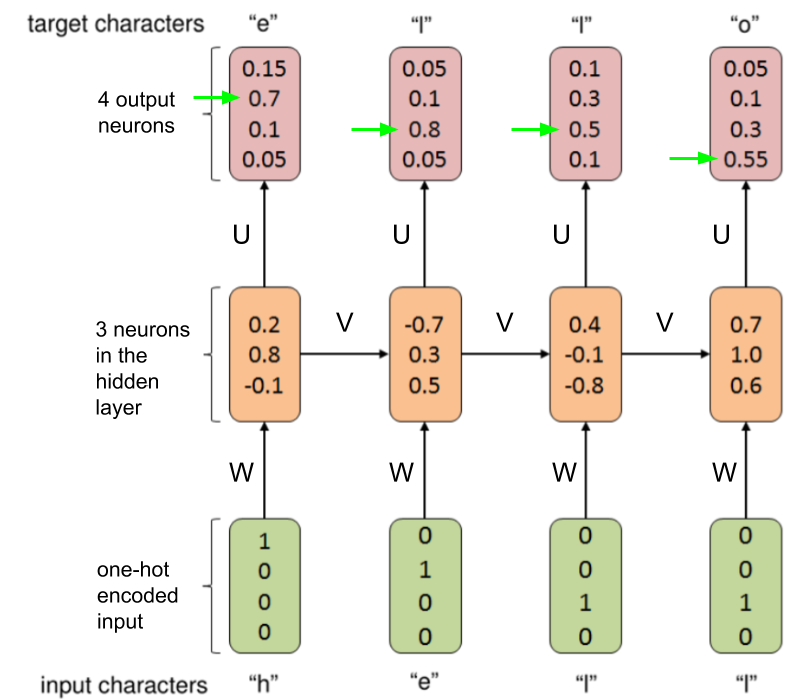
\includegraphics[width=6.5cm]{plots/m2many5.png}}%
  \end{figure}
  \begin{itemize}
    \only<1>{\item[] The probability of \enquote{e} should be high, given the context of \enquote{h}.} 
    \only<2>{\item[] The probability of \enquote{l} should be high, given in the context of \enquote{he}.} 
    \only<3>{\item[] The probability of \enquote{l} should \textbf{also} be high, given in the context of \enquote{hel}.}
    \only<4>{\item[] The probability of \enquote{o} should be high, given the context of \enquote{hell}.}
    \only<5>{\item[] During training, our goal would be to increase the confidence for the correct letters (indicated by the green arrows) and decrease the confidence of all others.}
  \end{itemize}
}
%%%%%%%%%%%%%%%%%%%%%%%%%%%%%%%%%%%%%%%%%%%%%%%%%%%%%%%%%%%%%%%%%%
%%%%%%%%%%%%%%%%%%%%%%%%%%%%%%%%%%%%%%%%%%%%%%%%%%%%%%%%%%%%%%%%%%
% \frame{
% \frametitle{RNNs - Generate sequences}
% 
% The RNN has a 4-dimensional input and output. The exemplary hidden layer consists of 3 neurons. This diagram shows the activations in the forward pass when the RNN is fed the characters \enquote{hell} as input. The output contains confidences the RNN assigns for the next character.
%   \begin{itemize}
%     \item[]
%   \end{itemize}
%   \begin{minipage}{0.55\textwidth}
%     \begin{figure}
%         \only<1>{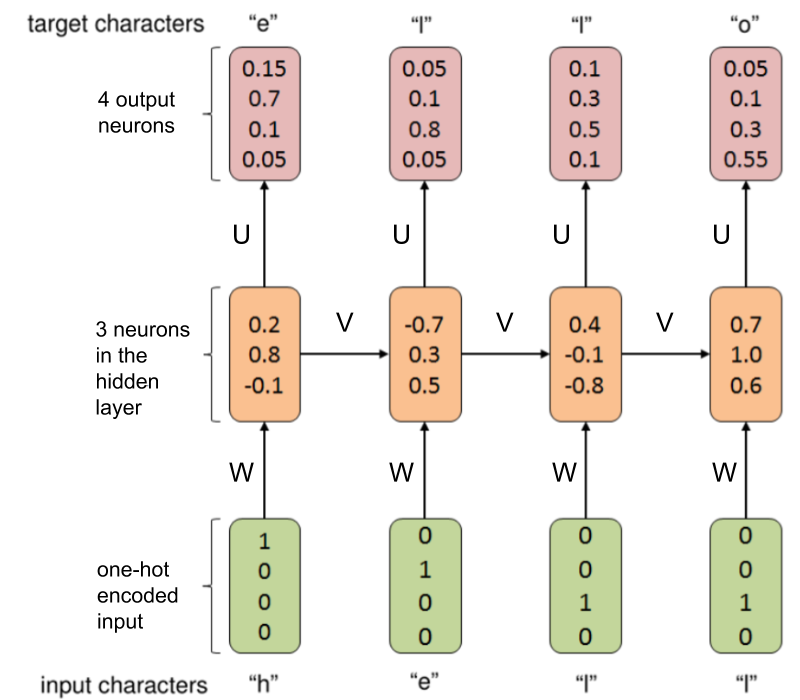
\includegraphics[width=5.5cm]{plots/m2many4.png}}%
%         \only<2>{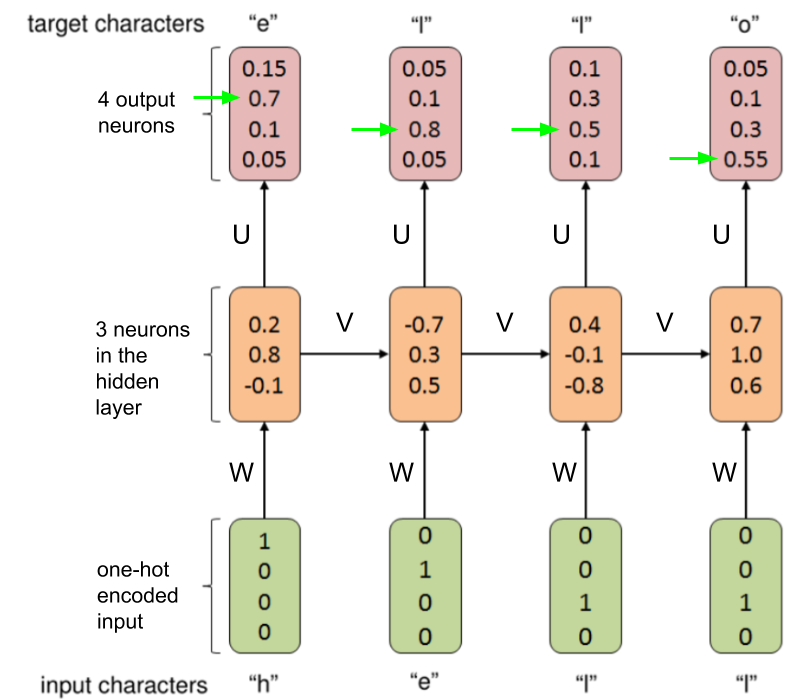
\includegraphics[width=5.5cm]{plots/m2many5.png}}%
%     \end{figure}
%   \end{minipage}%\hfill
%   \begin{minipage}{0.45\textwidth}
%   %\vspace{-0.3cm}
%   
%     \begin{itemize}
%       \only<1>{\item[] \textcolor{white}{Our goal is to increase the confidence for the correct letters (green digits) and decrease the confidence of all others.}} 
%       \only<2>{\item[] During training, our goal would be to increase the confidence for the correct letters (green digits) and decrease the confidence of all others.} 
%     \end{itemize}
%   \end{minipage}
% }
%%%%%%%%%%%%%%%%%%%%%%%%%%%%%%%%%%%%%%%%%%%%%%%%%%%%%%%%%%%%%%%%%%
%%%%%%%%%%%%%%%%%%%%%%%%%%%%%%%%%%%%%%%%%%%%%%%%%%%%%%%%%%%%%%%%%%
%\begin{frame} {Sentiment Neuron}
%  \begin{itemize}
%    \item \small {In 2017, a team at OpenAI trained a (more sophisticated) RNN to predict the next character in Amazon reviews.
%    \item The model had 4096 units in its hidden state and was trained on 82 million Amazon reviews.
%    \begin{figure}
%      \centering
%      \scalebox{0.5}{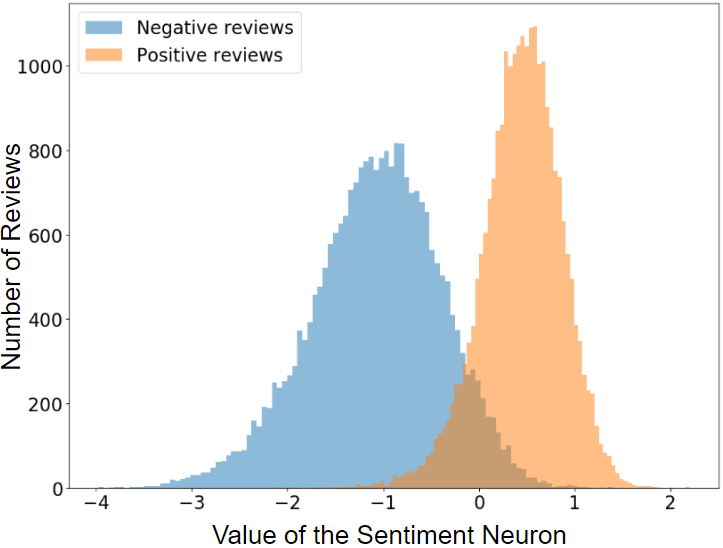
\includegraphics{plots/sent1b.png}}
%      \tiny{\\credit: OpenAI}
%  \end{figure}
%    \item To their surprise, one of the units had learned to detect the sentiment in the reviews extremely well even though the model was trained to only predict the next character in the text. In other words, the training data did not contain any explicit information regarding the sentiment.}
%  \end{itemize}
%\end{frame}
%
%\begin{frame} {Sentiment Neuron}
%  \begin{figure}
%      \centering
%      \scalebox{1}{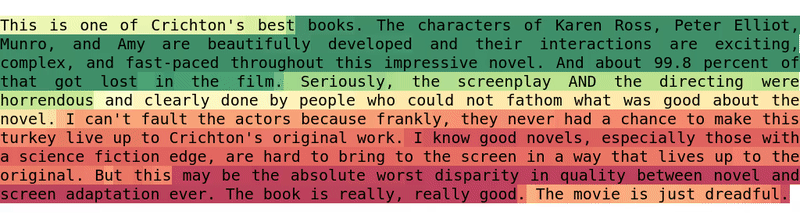
\includegraphics{plots/sent2.png}}
%      \tiny{\\credit: OpenAI}
%      \caption{\footnotesize {The background color of each character represents the activation of the sentiment neuron for that character. Positive values are green and negative values are red. }}
%  \end{figure}
%  
%  As the passage is fed to the RNN one character at a time, the activation of the sentiment neuron changes from a high value to a low value. Note the sharp jump in the activation after the word 'best' is fed to the network!
%\end{frame}
%%%%%%%%%%%%%%%%%%%%%%%%%%%%%%%%%%%%%%%%%%%%%%%%%%%%%%%%%%%%%%%%%%
%%%%%%%%%%%%%%%%%%%%%%%%%%%%%%%%%%%%%%%%%%%%%%%%%%%%%%%%%%%%%%%%%%
\begin{vbframe} {Word embeddings}
\begin{figure}
\vspace{-0.5cm}
      \centering
      \captionsetup{font=footnotesize,labelfont=footnotesize, labelfont = bf}
      \scalebox{0.65}{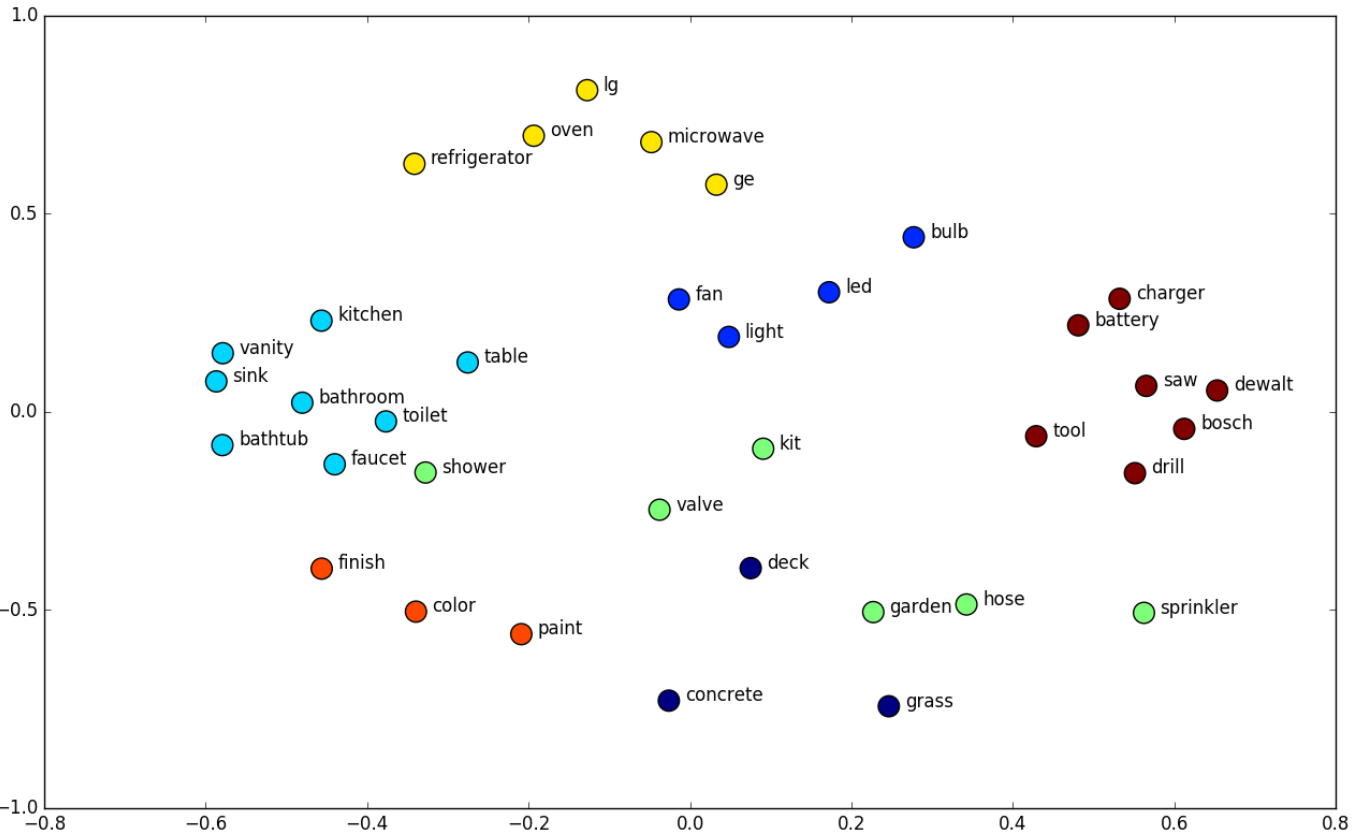
\includegraphics{plots/embed1.png}}
      \tiny{\\Source: Kaggle}
      \caption{\footnotesize{Two-dimensional embedding space. Typically, the embedding space is much higher dimensional.}}
      \vspace{-0.7cm}
        \end{figure}
  \begin{itemize}
    \item Instead of one-hot representations of words it is standard practice to encode each word as a dense (as opposed to sparse) vector of fixed size that captures its underlying semantic content.
    \item Similar words are embedded close to each other in a lower-dimensional embedding space. 
                \framebreak
    \item  The dimensionality of these embeddings is typically \text{much} smaller than the number of words in the dictionary. 
    \item Using them gives you a "warm start" for any NLP task. It is an easy way to incorporate prior knowledge into your model and a rudimentary form of \textbf{transfer learning}. 
    \item Two very popular approaches to learn  word embeddings are \textbf{word2vec} by Google and \textbf{GloVe} by Facebook. These embeddings are typically 100 to 1000 dimensional.
    \item Even though these embeddings capture the meaning of each word to an extent, they do not capture the \textit{semantics} of the word in a given context because each word has a static precomputed representation. For example, depending on the context, the word "bank" might refer to a financial institution or to a river bank.
    %     \item Recently, there have been significant breakthroughs in context-based embeddings. One such example are the embeddings provided by BERT [Devlin et al., 2018], a \textbf{transformer model} which was trained on a corpus of 3.3 billion words.
%     \item BERT (a non-recurrent model!) obtained new state-of-the-art performance on 11 NLP tasks.
  \end{itemize}
\end{vbframe}


%%%%%%%%%%%%%%%%%%%%%%%%%%%%%%%%%%%%%%%%%%%%%%%%%%%%%%%%%%%%%%%%%%
% \section{Bidirectional RNNs}
% 
% 
% \begin{vbframe}{Bidirectional RNNs}
%   \begin{itemize}
%     \item Another generalization of the simple RNN are bidirectional RNNs.
%     \item These allow us to process sequential data depending on both past and future inputs, e.g. an application predicting missing words, which probably depend on both preceding and following words.
%     \item One RNN processes inputs in the forward direction from $x^{[1]}$ to $x^{[T]}$ computing a sequence of hidden states $(z^{[1]}, \dots, z^{(T)})$, another RNN in the backward direction from $x^{[T]}$ to $x^{[1]}$ computing hidden states $(g^{[T]}, \dots, g^{[1]})$
%     \item Predictions are then based on both hidden states, which could be \textbf{concatenated}.
%     \item With connections going back in time, the whole input sequence must be known in advance
% to train and infer from the model.
%     \item Bidirectional RNNs are often used for the encoding of a sequence in machine translation.
%   \end{itemize}
% \framebreak  
% \textbf{Computational graph of an bidirectional RNN:}
%   \begin{figure}
%     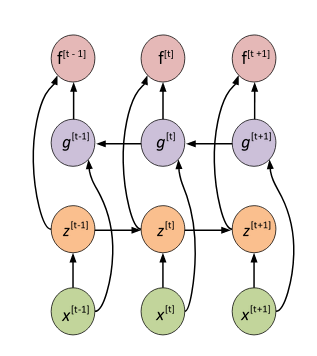
\includegraphics[width=4.5cm]{plots/bi_rnn.png}
%     \caption{A bidirectional RNN consists of a forward RNN processing inputs from left to right
% and a backward RNN processing inputs backwards in time.}
%   \end{figure} 
% \end{vbframe}



\section{Encoder-Decoder Architectures}


\begin{frame}


\vspace{15mm}
\hspace{25mm} \textbf{\LARGE{Seq-to-Seq (Type II)}}
\begin{figure}
      \centering
      \scalebox{0.9}{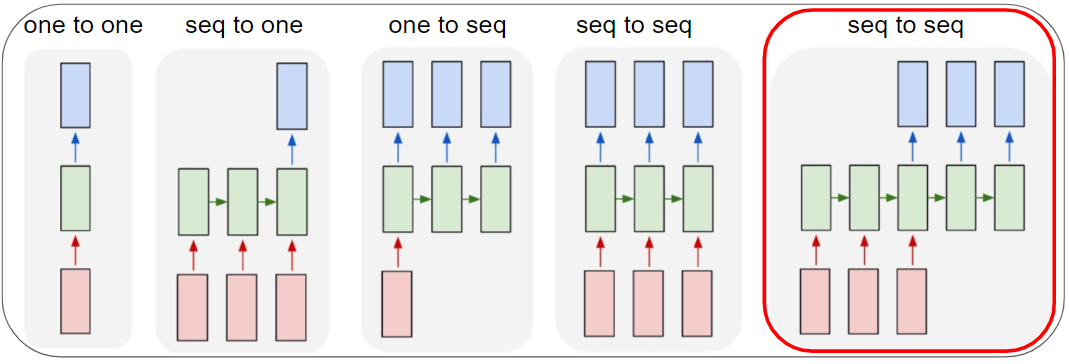
\includegraphics{plots/usecase_3.png}}
      \tiny{\\Credit: Andrej Karpathy}
  \end{figure}
  
\end{frame}

%%%%%%%%%%%%%%%%%%%%%%%%%%%%%%%%%%%%%%%%%%%%%%%%%%%%%%%%%%%%%%%%%%
\begin{vbframe}{Encoder-Decoder Network}
  \begin{itemize}
   % \item Standard RNNs operate on input and output sequences of the same length.
    \item For many interesting applications such as question answering, dialogue systems, or machine translation, the network needs to map an input sequence to an output sequence of different length.
    \item This is what an encoder-decoder (also called sequence-to-sequence architecture) enables us to do!
    
    \end{itemize}
 
 \framebreak
 
  \begin{figure}
    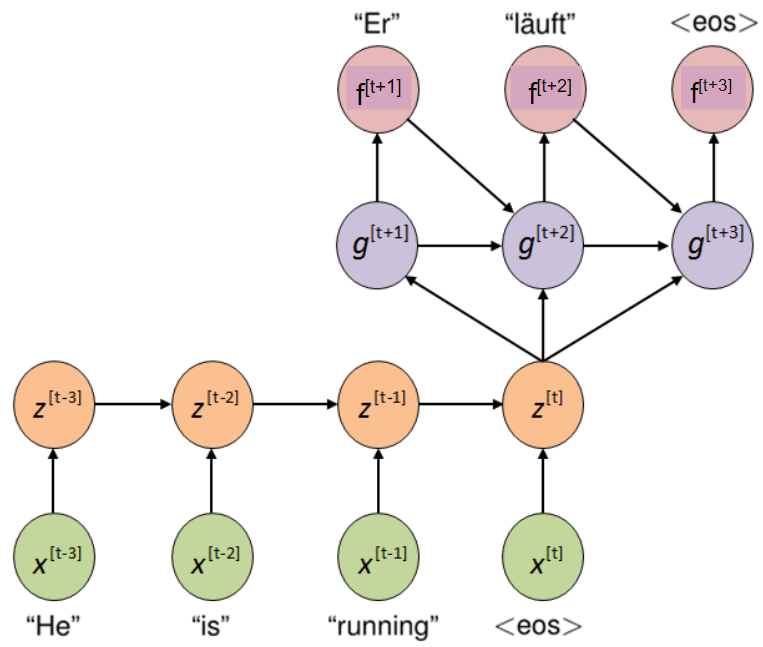
\includegraphics[width=7cm]{plots/seq2seq_2.png}
    \caption{%Encoder-decoder allows an RNN to process different length input and output sequences. 
    In the first part of the network, information from the input is encoded in the context vector, here the final hidden state, which is then passed on to every hidden state of the decoder, which produces the target sequence.}
  \end{figure} 
    
    
    \begin{itemize}
   
    \item An input/encoder-RNN processes the input sequence of length $n_x$ and computes a fixed-length context vector $C$, usually the final hidden state or  simple function of the hidden states.
    \item One time step after the other information from the input sequence is processed, added to the hidden state and passed forward in time through the recurrent connections between hidden states in the encoder.
    \item  The context vector summarizes important information from the input sequence, e.g. the intent of a question in a question answering task or the meaning of a text in the case of machine translation.
    \item The decoder RNN uses this information to predict the output, a sequence of length $n_y$, which could vary from $n_x$. 
    \item In machine translation, the decoder is a language model with recurrent connections between the output at one time step and the hidden state at the next time step as well as recurrent connections between the hidden states:
    $$\P(y^{[1]}, \dots, y^{[y_n]}|\xv^{[1]}, \dots, \xv^{[x_n]}) = \displaystyle \prod_{t=1}^{n_y} p(y^{[t]}|C; y^{[1]}, \dots, y^{[t-1]})$$ with $C$ being the context-vector.
    \item This architecture is now jointly trained to minimize the translation
error given a source sentence.
    \item Each conditional probability is then $$p(y^{[t]}|y^{[1]}, \dots, y^{[t-1]};C) = f(y^{[t-1]}, g^{[t]}, C)$$ where $f$ is a non-linear function, e.g. the tanh and $g^{[t]}$ is the hidden state of the decoder network.
 %   \item Encoder-decoder architectures are often used for machine translation, where they excel phrase-based translation models.
  \end{itemize}
%\framebreak
%  \begin{figure}
%    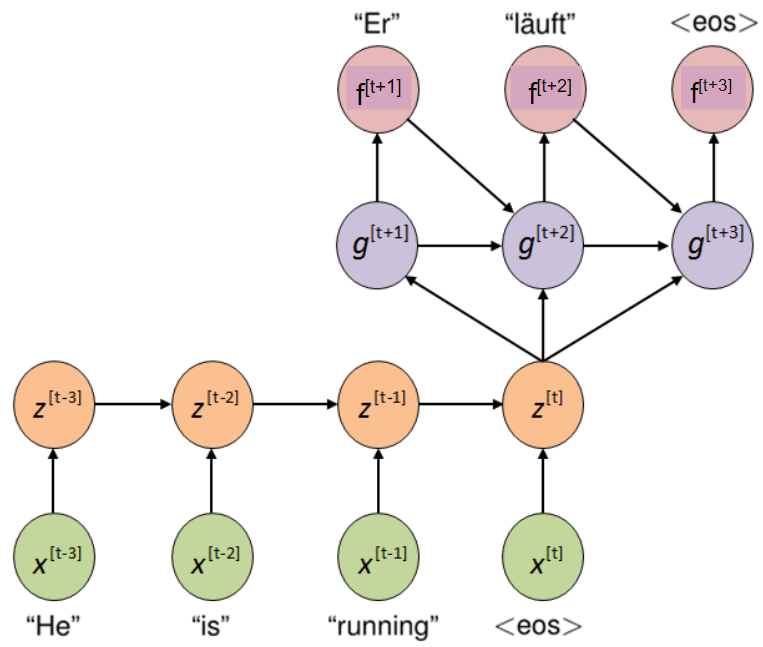
\includegraphics[width=7cm]{plots/seq2seq_2.png}
%    \caption{Encoder-decoder allows an RNN to process different length input and output sequences. In the first part of the network, information from the input is encoded in the context, here the final hidden state, which is then passed on to every hidden state of the decoder, which produces the target sequence.}
%  \end{figure} 
\end{vbframe}
%%%%%%%%%%%%%%%%%%%%%%%%%%%%%%%%%%%%%%%%%%%%%%%%%%%%%%%%%%%%%%%%%%
%%%%%%%%%%%%%%%%%%%%%%%%%%%%%%%%%%%%%%%%%%%%%%%%%%%%%%%%%%%%%%%%%%

\section{Attention}

\begin{vbframe}{Attention}
  \begin{itemize}
    \item In a classical decoder-encoder RNN all information about the input sequence must be incorporated into the final hidden state, which is then passed as an input to the decoder network.
    \item With a long input sequence this fixed-sized context vector is unlikely to capture all relevant information about the past.
      \item Each hidden state contains mostly information from recent inputs. 
      %In the case of a bidirectional RNN to encode the input sequence, a hidden state contains information from recent preceding and following inputs.
      \item Key idea: Allow the decoder to access all the hidden states of the encoder (instead of just the final one) so that it can dynamically decide which ones are relevant at each time-step of the decoding process.
      \item This means the decoder can choose to "focus" on different hidden states (of the encoder) at different time-steps of the decoding process similar to how the human eye can focus on different regions of the visual field.
      \item This is known as an \textbf{attention mechanism}.
   \end{itemize}
   
   \framebreak
   
   \begin{itemize}
      \item The attention mechanism is implemented by an additional component in the decoder.
      \item For example, this can be a simple single-hidden layer feed-forward neural network which is trained along with the RNN.
      \item At any given time-step $i$ of the decoding process, the network computes the relevance of encoder state $\bm{z}^{[j]}$ as:
            $$ rel(\bm{z}^{[j]})^{[i]} = \bm{v}_a^\top \text{tanh} (\bm{W}_a[\bm{g}^{[i-1]};\bm{z}^{[j]}]) $$
            where $\bm{v}_a$ and $\bm{W}_a$ are the parameters of the feed-forward network, $\bm{g}^{[i-1]}$ is the decoder state from the previous time-step and ';' indicates concatenation.
      %\item $v_a$ and $W_a$ are also learned through backpropagation.
      \item The relevance scores (for all the encoder hidden states) are then normalized which gives the \textit{attention weights} $(\alpha^{[j]})^{[i]}$:      
        $$ (\alpha^{[j]})^{[i]} = \frac{\exp (rel(\bm{z}^{[j]})^{[i]})}{\sum_{j'} \exp(rel(\bm{z}^{[j']})^{[i]})} $$
   \end{itemize}
   
   \framebreak
   
   \begin{itemize}  
    \item The attention mechanism allows the decoder network to focus on different parts of the input sequence by adding connections from all hidden states of the encoder to each hidden state of the decoder.
  %  \item At each point in time, a set of weights is computed which determine how to combine the hidden states of the encoder into a context vector $c_i$, which holds the necessary information to predict the correct output.
 %   \item Each hidden state contains mostly information from recent inputs. In the case of a bidirectional RNN to encode the input sequence, a hidden state contains information from recent preceding and following inputs.
  \end{itemize}
 \begin{figure}
    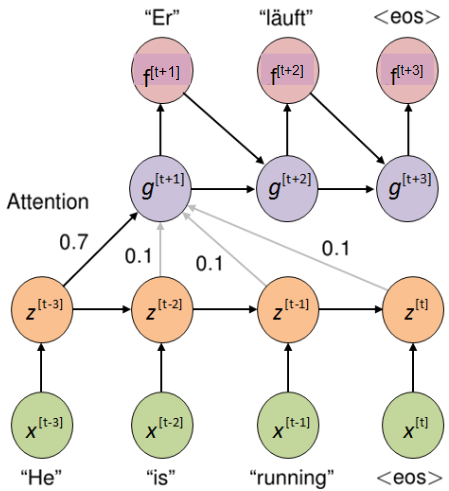
\includegraphics[width=4.cm]{plots/seq2seq_3.png}
    \caption{Attention at $i=t+1$}
  \end{figure}
 
\framebreak
\begin{itemize}  
   % \item An \textbf{attention mechanism} allows the decoder network to focus on different parts of the input sequence by adding connections from all hidden states of the encoder to each hidden state of the decoder
    \item At each time step $i$, a set of weights $(\alpha^{[j]})^{[i]}$ is computed which determine how to combine the hidden states of the encoder into a context vector $c^{[i]}= \sum_{j=1}^{n_x} (\alpha^{[j]})^{[i]} \bm{z}^{[j]}$, which holds the necessary information to predict the correct output.
 %   \item Each hidden state contains mostly information from recent inputs. In the case of a bidirectional RNN to encode the input sequence, a hidden state contains information from recent preceding and following inputs.
  \end{itemize}
  \begin{figure}
    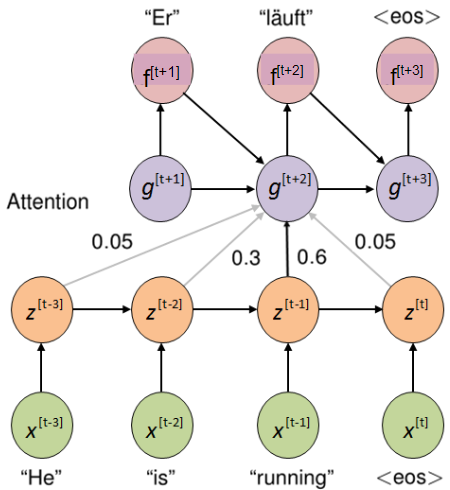
\includegraphics[width=4.cm]{plots/seq2seq_4.png}
    \caption{Attention at $i=t+2$}
  \end{figure}
  
\framebreak
  
  \lz
  \lz
  \begin{figure}
    \centering
    \scalebox{0.9}{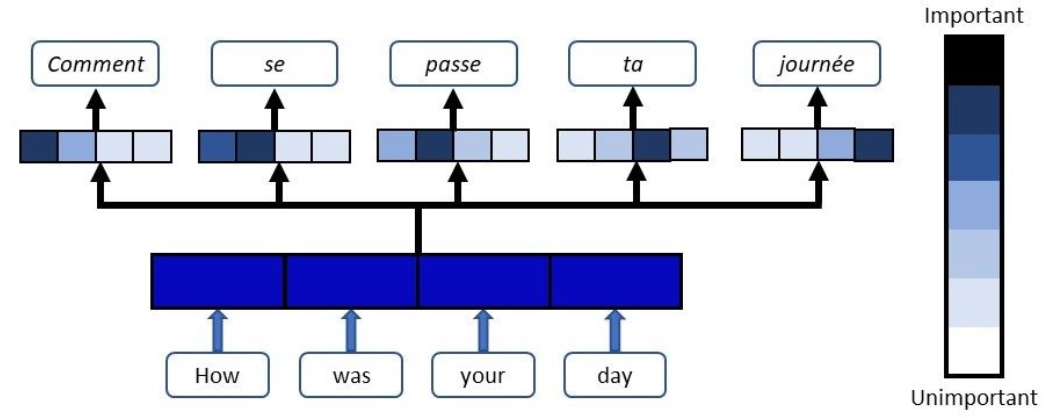
\includegraphics{plots/attention_example.png}}
    \tiny{\\Credit: Gabriel Loye}
    \caption{\footnotesize An illustration of a machine translation task using an encoder-decoder model with an attention mechanism. The attention weights at each time-step of the decoding/translation process indicate which parts of the input sequence are most relevant. (There are 4 attention weights because there are 4 encoder states.)}
  \end{figure}
\end{vbframe}

\begin{vbframe}{Transformers}
  \begin{itemize}
    \item Advanced RNNs have similar limitations as vanilla RNN network.
    \begin{itemize}
      \item Lack of parallelization, RNNs process the input data sequentially, as the output of a step depends on the output of the previous step.
     \item Difficulties in learning long term dependency, Although GRU or LSTM perform superior compared to vanilla RNN, even they struggle to remember the context from a word which stands much earlier in long sequences.
    \end{itemize}
    \item These challenges are successfully tackled by transformer networks.
    
    \framebreak
    
    \item Transformers are solely based on attention (no RNN or CNN).
    \item In fact, the paper which coined the term \textit{transformer} is called \textit{Attention is all you need}.
    \item They are the state-of-the-art networks in natural language processing (NLP) tasks since 2017.
    \item Transformer architectures like BERT (Bidirectional Encoder Representations from Transformers, 2018) and GPT-3 (Generative Pre-trained Transformer-3, 2020) are pre-trained in a large text and can be fine-tuned (quickly adapt) to specific language tasks.
  \end{itemize}
\end{vbframe}





%%%%%%%%%%%%%%%%%%%%%%%%%%%%%%%%%%%%%%%%%%%%%%%%%%%%%%%%%%%%%%%%%%
%%%%%%%%%%%%%%%%%%%%%%%%%%%%%%%%%%%%%%%%%%%%%%%%%%%%%%%%%%%%%%%%%%
%\section{Neural Turing Machines}
%
%\begin{frame} {Neural Turing Machines}
%  \begin{itemize}
%    \item We've seen that an RNN has a form of \textbf{internal} "short-term memory" that enables it to process inputs sequentially.
%    \item In 2014, a team at DeepMind [Graves et al. , 2014] introduced the 'Neural Turing Machine (NTM) ' which combines an RNN with an \textbf{external} memory bank.
%    \item This external memory bank is just a real valued matrix.
%    \item The NTM has an \textbf{attention mechanism} which enables the RNN to read from and write to the external memory.
%    \item It's helpful to think of the RNN as the 'processor' and the memory bank as the 'RAM' in a computer.
%    \item Importantly, the \textit{whole} system is end-to-end trainable by gradient descent. That is, the network eventually learns where to read and write to perform the task.
%  \end{itemize}
%\end{frame}
%
%% Here's a great blog article from which the images below were taken : https://distill.pub/2016/augmented-rnns/
%
%\begin{frame} {Neural Turing Machines}
%  \begin{figure}
%      \centering
%      \scalebox{1.1}{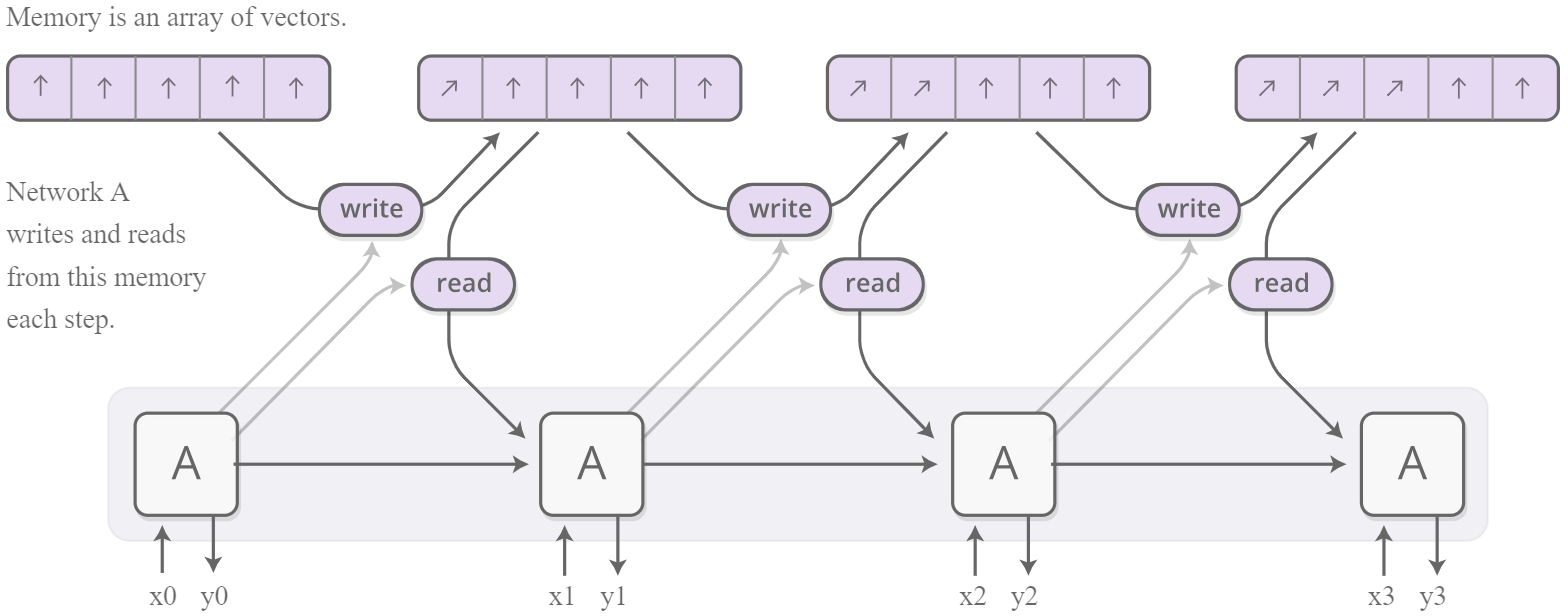
\includegraphics{plots/ntm2.png}}
%      \tiny{\\credit: Chris Olah}
%      \caption{\footnotesize{The Neural Turing Machine architecture.}}
%  \end{figure}
%    Like any RNN, the controller (network 'A') is fed input vectors and produces output vectors. However, unlike a typical RNN, the controller also reads from and writes to the external memory.
%\end{frame}
%
%\begin{frame} {Neural Turing Machines}
%  \begin{figure}
%      \centering
%      \scalebox{1}{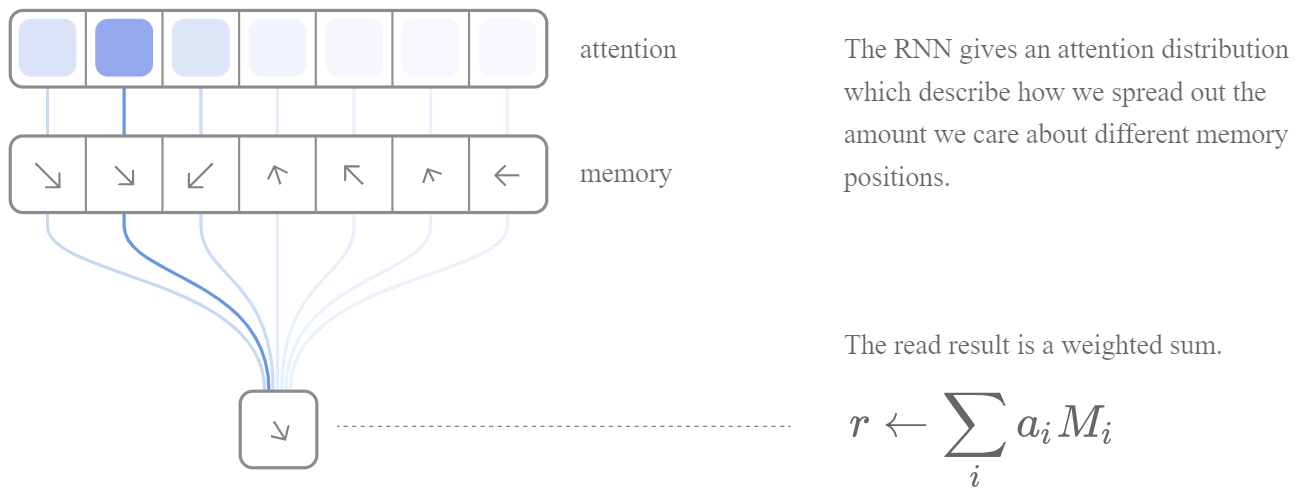
\includegraphics{plots/ntm1.png}}
%      \tiny{\\credit: Chris Olah}
%      \caption{\footnotesize{An illustration of the 'read' operation in an NTM.}}
%  \end{figure}
%  
%  $M_i$ is the memory vector in the $i$-th location and $a_i$ is the associated attention weight. The value that is read from the memory matrix is a convex combination of all the vectors in the matrix.
%\end{frame}


\section{More application examples}

\frame{
\frametitle{Some more sophisticated applications}
  \begin{figure}
      \only<1>{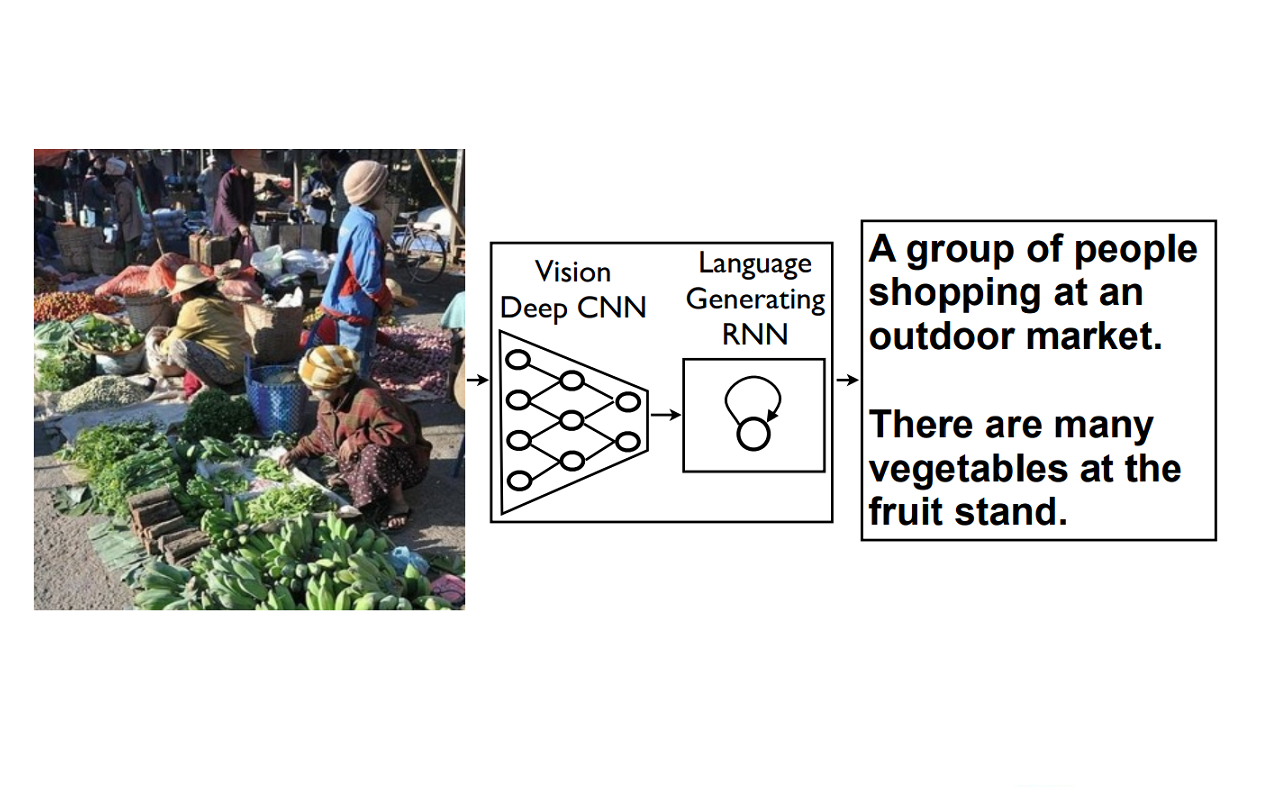
\includegraphics[width=9.5cm]{plots/image_caption2.png}}%
      \only<2>{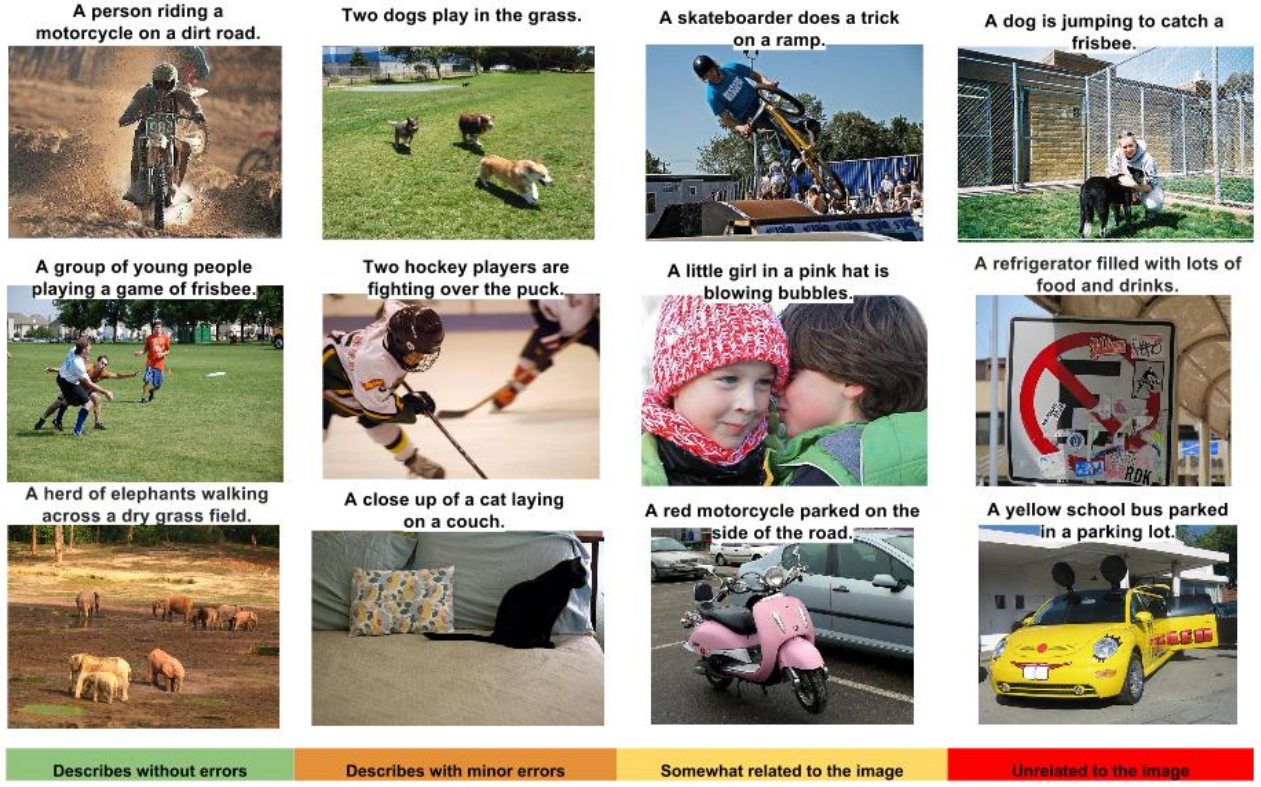
\includegraphics[width=9.5cm]{plots/image_caption.png}}%
  \end{figure}
\textbf{Figure:} Show and Tell: A Neural Image Caption Generator (Oriol Vinyals et al. 2014). A language generating RNN tries to describe in brief the content of different images.
}
%%%%%%%%%%%%%%%%%%%%%%%%%%%%%%%%%%%%%%%%%%%%%%%%%%%%%%%%%%%%%%%%%%
\frame{
\frametitle{Some more sophisticated applications}
  \begin{figure}
    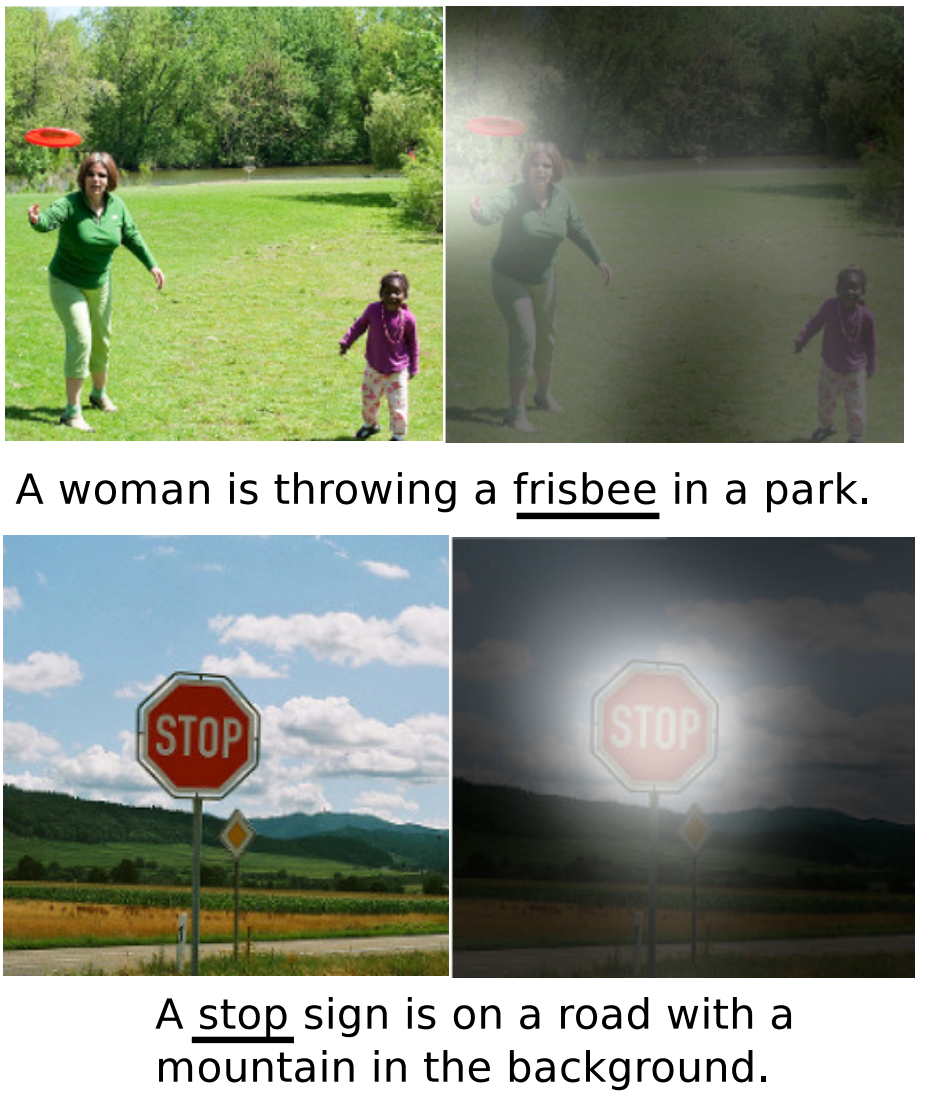
\includegraphics[width=5cm]{plots/attention3.png}
    \caption{Attention for image captioning: the attention mechanism tells the network roughly which pixels to pay attention to when writing the text (Kelvin Xu al. 2015)}
  \end{figure}
}
%%%%%%%%%%%%%%%%%%%%%%%%%%%%%%%%%%%%%%%%%%%%%%%%%%%%%%%%%%%%%%%%%%
\frame{
\frametitle{Some more sophisticated applications}
  \begin{figure}
      \only<1>{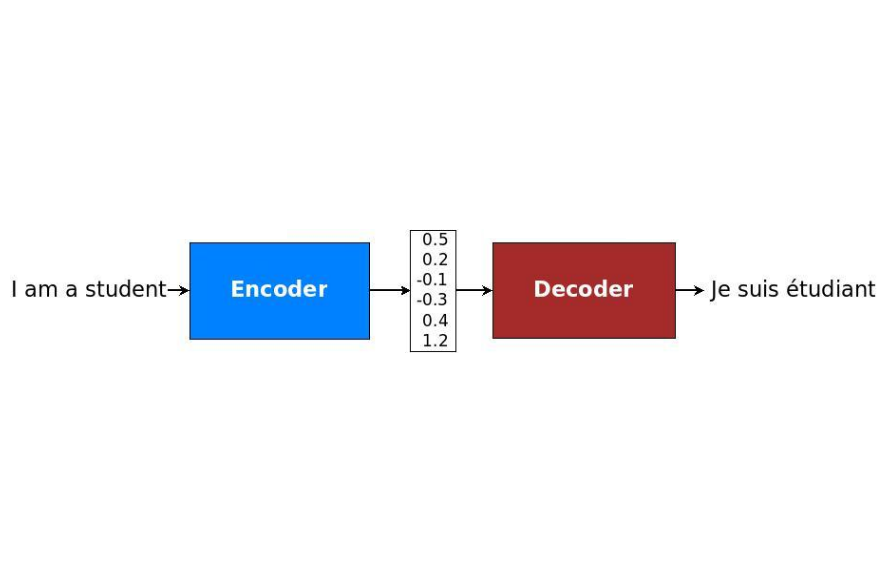
\includegraphics[width=8.5cm]{plots/seq2seq.png}}%
      \only<2>{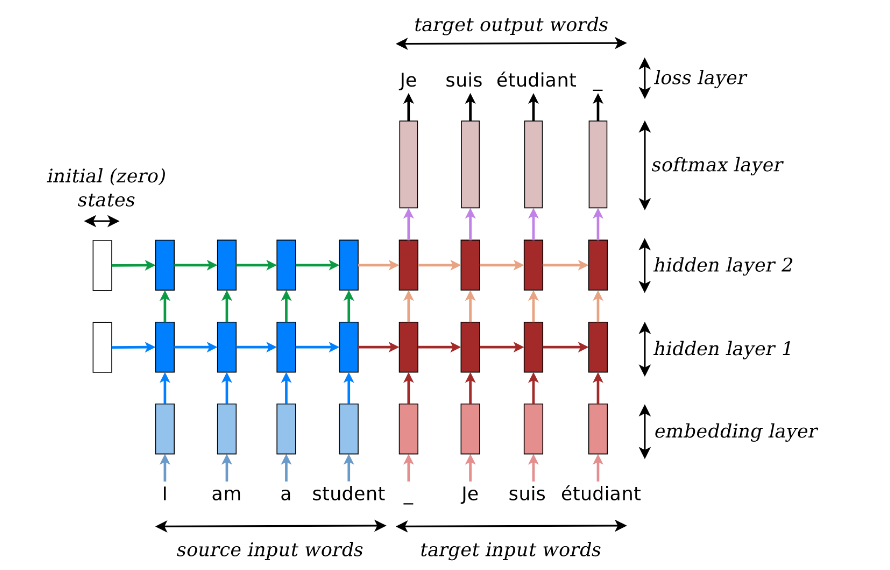
\includegraphics[width=8.5cm]{plots/seq2seq2.png}}%
  \end{figure}
\textbf{Figure:} Neural Machine Translation (seq2seq): Sequence to Sequence Learning with Neural Networks (Ilya Sutskever et al. 2014). As we saw earlier, an encoder converts a source sentence into a \enquote{meaning} vector which is passed through a decoder to produce a translation.
}
%%%%%%%%%%%%%%%%%%%%%%%%%%%%%%%%%%%%%%%%%%%%%%%%%%%%%%%%%%%%%%%%%%
%%%%%%%%%%%%%%%%%%%%%%%%%%%%%%%%%%%%%%%%%%%%%%%%%%%%%%%%%%%%%%%%%%
\begin{vbframe}{Some more sophisticated applications}
  \begin{figure}
    \centering
    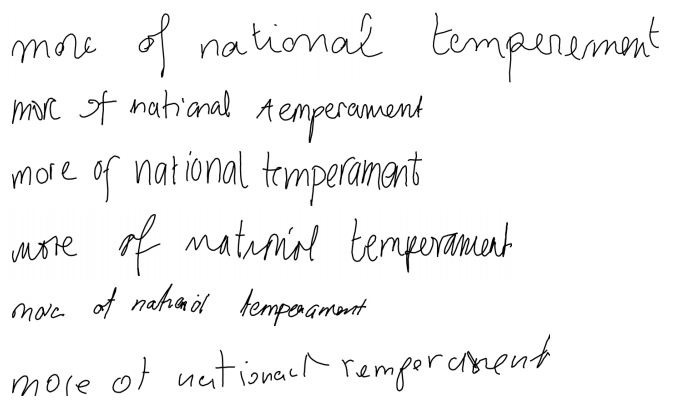
\includegraphics[width=10cm]{plots/hand_writing_generation.png}
    \caption{Generating Sequences With Recurrent Neural Networks (Alex Graves, 2013). Top row are real data, the rest are generated by various RNNs.}
  \end{figure}
\framebreak
  \begin{figure}
    \centering
    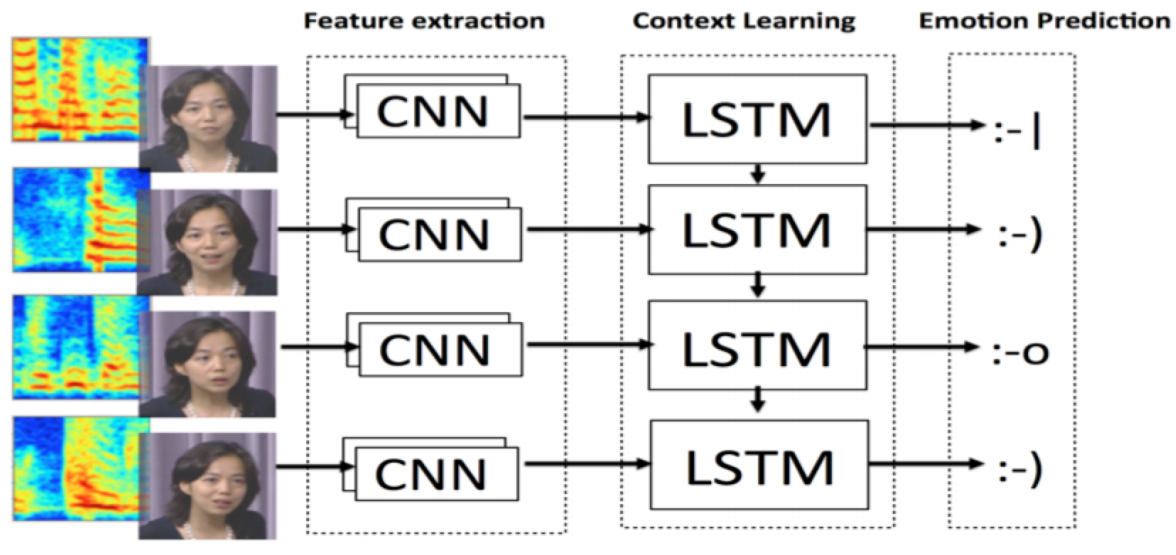
\includegraphics[width=11.5cm]{plots/emotion_from_audio_data.png}
    \caption{Convolutional and recurrent nets for detecting emotion from audio data (Namrata Anand \& Prateek Verma, 2016). We already had this example in the CNN chapter!}
  \end{figure}  
\framebreak
  \begin{figure}
    \centering
    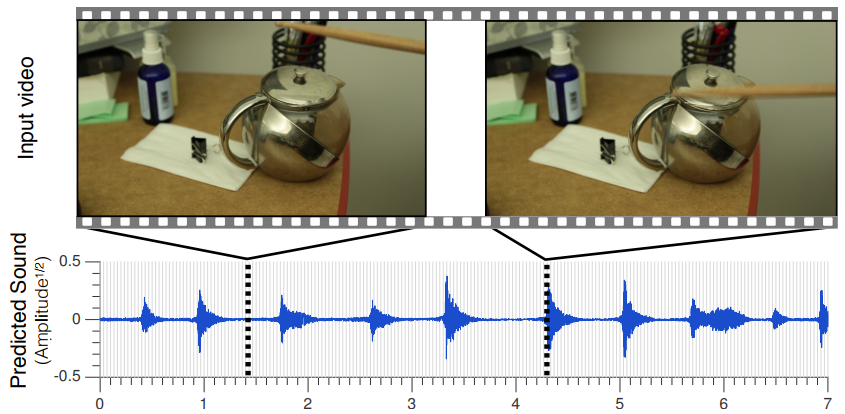
\includegraphics[width=11.5cm]{plots/visually_indicated_sounds.png}
    \caption{Visually Indicated Sounds (Andrew Owens et al. 2016). A model to synthesize plausible impact sounds from silent videos.\href{https://www.youtube.com/watch?v=0FW99AQmMc8&feature=youtu.be&t=61}{\beamergotobutton{Click here}}}
  \end{figure}   
\end{vbframe}
%%%%%%%%%%%%%%%%%%%%%%%%%%%%%%%%%%%%%%%%%%%%%%%%%%%%%%%%%%%%%%%%%%
%%%%%%%%%%%%%%%%%%%%%%%%%%%%%%%%%%%%%%%%%%%%%%%%%%%%%%%%%%%%%%%%%%
%%%%%%%%%%%%%%%%%%%%%%%%%%%%%%%%%%%%%%%%%%%%%%%%%%%%%%%%%%%%%%%%%%
%%%%%%%%%%%%%%%%%%%%%%%%%%%%%%%%%%%%%%%%%%%%%%%%%%%%%%%%%%%%%%%%%%

\section{CNNs or RNNs?}

\begin{frame} {CNNs or RNNs?}
  \begin{itemize}
    \item Historically, RNNs were the default models used in sequence processing tasks.
    \item However, some families of CNNs (especially those based on Fully Convolutional Networks (FCNs)) \textit{can} be used to process variable-length sequences such as text or time-series data.
    \item If a CNN doesn't contain any fully-connected layers, the total number of weights in the network is independent of the spatial dimensions of the input because of weight-sharing in the convolutional layers.
    \item Recent research [Bai et al. , 2018] indicates that such convolutional architectures (which the authors term Temporal Convolutional Networks (TCNs)) can outperform RNNs on a wide range of tasks.
    \item A major advantage of TCNs is that the entire input sequence can be fed to the network at once (as opposed to sequentially).
    % \item Surprisingly, the TCNs can model long-range dependencies in the inputs even better than recurrent architectures!
  \end{itemize}
\end{frame}

\begin{frame} {CNNs or RNNs?}
  \begin{figure}
      \centering
      \scalebox{1}{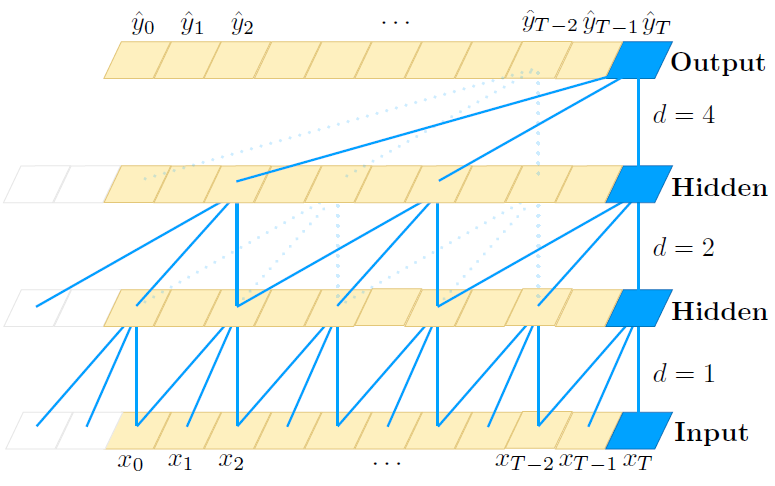
\includegraphics{plots/tcn2.png}}
      \caption{\footnotesize{A TCN (we have already seen this in the CNN lecture!) is simply a variant of the one-dimensional FCN which uses a special type of dilated convolutions called \textbf{causal dilated} convolutions.}}
  \end{figure}
\end{frame}


\begin{frame} {CNNs or RNNs?}
  \begin{figure}
      \centering
      \scalebox{1}{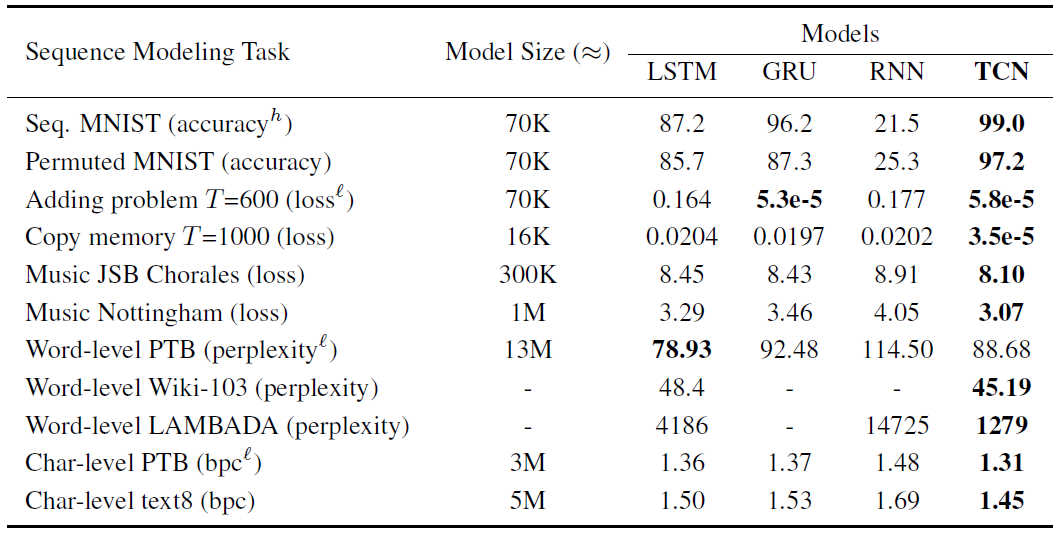
\includegraphics{plots/tcn1.png}}
      \caption{\footnotesize{Evaluation of TCNs and recurrent architectures on a wide range of sequence modelling tasks. $^h$ means higher is better and ${}^\ell$~ means lower is better. Note: To make the comparisons fair, all models have roughly the same size (for a given task) and the authors used grid search to find good hyperparameters for the recurrent architectures.}}
  \end{figure}
\end{frame}


\begin{frame}{Summary}
\begin{itemize}
\item RNNs are specifically designed to process sequences of varying lengths. 
\item  For that recurrent connections are introduced into the network structure.
\item The gradient is calculated by backpropagation through time.
\item  An LSTM replaces the  simple hidden neuron by a complex system consisting of cell state, and forget, input, and output gates.
\item An RNN can be used as a language model, which can be improved by word-embeddings.
\item Different advanced types of RNNs exist, like Encoder-Decoder architectures and bidirectional RNNs.$^1$
\end{itemize}

\vspace{8mm}
\tiny{1. A bidirectional RNN processes the input sequence in both directions (front-to-back and back-to-front).}

\end{frame}

%%%%%%%%%%%%%%%%%%%%%%%%%%%%%%%%%%%%%%%%%%%%%%%%%%%%%%%%%%%%%%%%%%
%%%%%%%%%%%%%%%%%%          REFERENCES          %%%%%%%%%%%%%%%%%%
%%%%%%%%%%%%%%%%%%%%%%%%%%%%%%%%%%%%%%%%%%%%%%%%%%%%%%%%%%%%%%%%%%
\begin{vbframe}
\frametitle{References}
\footnotesize{
\begin{thebibliography}{99}
%%%%%%%%%%%%%%%%%%%%%%%%%%%%%%%%%%
\bibitem[Ian Goodfellow et al., 2016]{1} Ian Goodfellow, Yoshua Bengio and Aaron Courville (2016)
\newblock Deep Learning
\newblock \emph{\url{http://www.deeplearningbook.org/}}
%%%%%%%%%%%%%%%%%%%%%%%%%%%%%%%%%%
\bibitem[Oriol Vinyals et al., 2014]{2} Oriol Vinyals, Alexander Toshev, Samy Bengio and Dumitru Erhan (2014)
\newblock Show and Tell: A Neural Image Caption Generator
\newblock \emph{\url{https://arxiv.org/abs/1411.4555}}
%%%%%%%%%%%%%%%%%%%%%%%%%%%%%%%%%%
\bibitem[Alex Graves, 2013]{3} Alex Graves (2013)
\newblock Generating Sequences With Recurrent Neural Networks
\newblock \emph{\url{https://arxiv.org/abs/1308.0850}}
%%%%%%%%%%%%%%%%%%%%%%%%%%%%%%%%%%
\bibitem[Namrata Anand and Prateek Verma, 2016]{4} Namrata Anand and Prateek Verma (2016)
\newblock Convolutional and recurrent nets for detecting emotion from audio data
\newblock \emph{\url{http://cs231n.stanford.edu/reports/2015/pdfs/Cs_231n_paper.pdf}}
%%%%%%%%%%%%%%%%%%%%%%%%%%%%%%%%%%
\bibitem[Gabriel Loye, 2019]{5} Gabriel Loye (2019)
\newblock Attention Mechanism
\newblock \emph{\url{https://blog.floydhub.com/attention-mechanism/}}
%%%%%%%%%%%%%%%%%%%%%%%%%%%%%%%%%%
\bibitem[Andrew Owens et al., 2016]{6} Andrew Owens, Phillip Isola, Josh H. McDermott, Antonio Torralba, Edward H. Adelson and  William T. Freeman (2015)
\newblock Visually Indicated Sounds
\newblock \emph{\url{https://arxiv.org/abs/1512.08512}}
%%%%%%%%%%%%%%%%%%%%%%%%%%%%%%%%%%
%%%%%%%%%%%%%%%%%%%%%%%%%%%%%%%%%%
\bibitem[Andrej Karpathy., 2015]{7} Andrej Karpathy (2015)
\newblock The Unreasonable Effectiveness of Recurrent Neural Networks
\newblock \emph{\url{http://karpathy.github.io/2015/05/21/rnn-effectiveness/}}
% \bibitem[Devlin et al., 2018]{7} Jacob Devlin, Ming-Wei Chang, Kenton Lee, Kristina Toutanova (2018)
% \newblock BERT: Pre-training of Deep Bidirectional Transformers for Language Understanding
% \newblock \emph{\url{https://arxiv.org/abs/1810.04805}}
%%%%%%%%%%%%%%%%%%%%%%%%%%%%%%%%%%
\bibitem[Kelvin Xu al., 2016]{8} Kelvin Xu, Jimmy Ba, Ryan Kiros, Kyunghyun Cho, Aaron C. Courville, Ruslan Salakhutdinov, Richard S. Zemel and  Yoshua Bengio (2015)
\newblock Show, Attend and Tell: Neural Image Caption Generation with Visual Attention
\newblock \emph{\url{https://arxiv.org/abs/1502.03044}}
%%%%%%%%%%%%%%%%%%%%%%%%%%%%%%%%%%
\bibitem[Bai et al., 2018]{9} Shaojie Bai, J. Zico Kolter, Vladlen Koltun (2018)
\newblock An Empirical Evaluation of Generic Convolutional and Recurrent Networks for Sequence Modeling
\newblock \emph{\url{https://arxiv.org/abs/1803.01271}}
%%%%%%%%%%%%%%%%%%%%%%%%%%%%%%%%%%
\bibitem[Weng 2018]{10} Lilian Weng (2018)
\newblock Attention? Attention!
\newblock \emph{\url{https://lilianweng.github.io/lil-log/2018/06/24/attention-attention.html}}
%%%%%%%%%%%%%%%%%%%%%%%%%%%%%%%%%%
\end{thebibliography}
}
\end{vbframe}
%%%%%%%%%%%%%%%%%%%%%%%%%%%%%%%%%%%%%%%%%%%%%%%%%%%%%%%%%%%%%%%%%%
%%%%%%%%%%%%%%%%%%%%%%%%%%%%%%%%%%%%%%%%%%%%%%%%%%%%%%%%%%%%%%%%%%

\endlecture
\end{document}
